\documentclass[journal, onecolumn]{IEEEtran}
\usepackage[utf8]{inputenc}

\usepackage{graphicx}
\usepackage{amsmath}
\usepackage{hyperref}
\usepackage{gensymb}
\usepackage{authblk}
\usepackage{caption}
\usepackage{xcolor}
\usepackage{subcaption}
\usepackage{cite}
\usepackage{float}
\usepackage{booktabs}
\usepackage[toc,page]{appendix}

\title{\bfseries Software Validation: A Literature Review\\ \Large CS300 Mini Project}

\author[1]{Drishika Nadella}	
\author[2]{Kriti Shukla}
\author[3]{Ramya Hegde}
\author[4]{Sudeepthi Nalla}

\affil[1]{181ME222, Department of Mechanical Engineering, NITK}
\affil[2]{181ME239, Department of Mechanical Engineering, NITK}
\affil[3]{181CV123, Department of Civil Engineering, NITK}
\affil[4]{181CV134, Department of Civil Engineering, NITK}

\date{26th March 2021}

\newcommand\todo[1]{\textcolor{red}{#1}}
\renewcommand\thesection{\arabic{section}}

\begin{document}
	
	\maketitle
	
	\begin{abstract}
		Software validation is a process that ensures that the developed software fulfills its intended purpose, satisfies the various requirements and is approved by the stakeholders. This literature review focuses on recent developments in the field of software validation. We review the various tools and technologies that are available for software validation today  and various forms of validation testing. We discuss Independent Verification and Validation (IV\&V) and a "Reference Model" for an efficient execution of IV\&V. The application of IV\&V in the agile life cycle model of software development is also discussed. We also analyse scaling algorithms for software validation. We evaluate the findings from the various papers, perform a comparison study and contrast the advantages and disadvantages in the various approaches given.
	\end{abstract}
	
	\tableofcontents
	\listoffigures
	\listoftables
	
	\section{Introduction}
	\bigskip
	
	Software Engineering is an engineering approach to software development, which uses a set of techniques, guidelines and methodologies to develop software from a set of requirements. It systematically allows for the development, operation and maintenance of software. A software project management involves a step-by-step procedure of developing software. It includes feasibility study, requirement specification, software design, coding and testing, integration and software verification and validation. 
	
	\begin{figure}[h]
		\includegraphics[scale=0.35]{process.jpg}
		\centering
		\caption{A generic lifecycle for a software development project}
	\end{figure}
	
	Software validation is a process that ensures that the developed software fulfills its intended purpose, satisfies the various requirements and is approved by the stakeholders. This literature review focuses on recent developments in the field of software validation. We describe the necessary background required in Section 2. We review the various tools and technologies that are available for software validation today \cite{tools} in Section 3-A and various forms of validation testing \cite{regression}\cite{trace}\cite{hazard} in Section 3-B. In Section 3-C, we discuss Independent Verification and Validation (IV\&V) \cite{ivv} and a 'Reference Model' for an efficient execution of IV\&V \cite{refmod} in Section 3-D. The application of IV\&V in the agile life cycle model of software development \cite{agile} is discussed in Section 3-E. We also analyse scaling algorithms for software validation \cite{ref:algo} in Section 3-F. In Section 4, we evaluate the findings from the various papers, perform a comparison study and contrast the advantages and disadvantages in the various approaches given.
	
	\section{Background}
	\bigskip
	The IEEE 1012 Standard for Verification and Validation (V{\&}V) defines software validation as the process of providing evidence that the system, software, or hardware and its associated products satisfy requirements allocated to it at the end of each life cycle activity, solve the right problem (e.g., correctly model physical laws, implement business rules, and use the proper system assumptions), and satisfy intended use and user needs \cite{standard}. Software validation is done to ensure that the software achieves its intended purpose and performs under several conditions. Validating the software regularly throughout the development process not only ensures that the right requirement specifications are followed, but also to make certain that no unintended features creep in. 
	\newline \newline
	During the software development process, verification and validation often occur simultaneously. However, developers often perform software verification extensively, but validation is not given the same level of importance. Verification ensures that the product is being built in the right way, but validation checks if the right product is being built. Another important difference between verification and validation is that, while verification only requires objective proof that the requirements specifications are met, validation also checks that the mission behind the software is achieved and requires stakeholder approval.
	\newline \newline
	The software validation process can happen through inspection, tests, analysis, simulations etc. Therefore, it is important to start the validation process early. Not only do test cases have to be developed, but it is possible that the software validation process may require special equipment or simulated environments. 
	\newline \newline
	Another important reason to start software validation early is the reduced cost of error detection and correction for regularly tested software. It was found that error detection and correction costs increase threefold from coding to the assembly phase, sevenfold in the testing and integration phase, 50 times in the trial phase and a 100 times more during the operational phase of the software \cite{chapter7}. Therefore, it is necessary to diligently perform software V\&V so as to detect and correct bugs in the same phase as their origin, hence reducing the costs associated with it.
	\newline \newline
	There are several other advantages of regular software validation. It results in:
	\begin{itemize}
		\item an early evaluation of performance
		\item upholding of the schedule and budget of the development process
		\item improves software quality
	\end{itemize}
	
	\section{Related Work}
	\bigskip
	\subsection{Software Validation Tools and Technologies}
	\bigskip
	Today, software projects are bigger and more complex than ever before. A study shows that about half of today's large scale software projects go 45\% over budget, 7\% over time and produce 56\% lesser valued projects than promised \cite{mckinsey}. In such an age, using the right tools and technologies for timely and effective software validation is imperative. 
	\newline \newline
	A software validation plan, written by a software manager, lists the organization and resources required to validate software. It also provides several test iterations, steps and objectives that need to be achieved. Some of these tests, tools and technologies are discussed in Rodriguez et al. \cite{tools}.
	\newline \newline
	Before choosing the right tools for validation of a software project, it is important to know the various software product characteristics that define software quality, according to ISO 25000 \cite{iso25000} series:
	\begin{itemize}
		\item \textbf{Functional suitability}: It defines the extent to which software functions meet their stated requirments.
		\item \textbf{Maintainability}: According to the changes in the environment, the degree of efficiency and effectiveness with which the software product can be improved or corrected by modifying it to adapt.
		\item \textbf{Usability}: In a specified context of use, the degree to which specified users can use the product to achieve the specified goals effectively defines its usability.
		\item \textbf{Security}: It is the degree to which a product protects information so that another person connected to this product will have their data protected with appropriate data access according to their authorisation.
		\item \textbf{Performance efficiency}: It represents the relative performance of the software product used under stated conditions to the amount of resources used.		
	\end{itemize}
	
	Keeping in mind the above software qualities, the right tests and tools for a software project validation can be implemented.
	
	\bigskip
	
	\subsubsection{Tests}
	
	The authors define four major types of tests in software validation:
	
	\begin{itemize}
		\item Development tests: According to ISO 24765 \cite{ISO24765}, the development test is conducted during the development of the system usually in the development environment in a formal or informal way by a developer.
		\item Acceptance tests: According to IEEE 829 \cite{ieee829}, this testing is done to check whether a software product satisfies the acceptance criteria and enables the consumer whether they should accept the product.
		\item Qualification tests: According to ISO 12207 \cite{iso12207}, the consumer's testing is witnessed while the developer tests to prove that a software product meets its specifications and is ready for use in a real environment.
		\item Operational tests: According to IEEE 829 \cite{ieee829}, the testing is conducted in the operational environment for evaluation.
	\end{itemize}
	\bigskip
	The tests can be automated with the help of certain technologies and tools. The efficiency of the V\&V process increases with the increase in automation. Some common testing methods such as regression testing, hazard analysis and traceability analysis are discussed in detail in the coming sections.
	
	\bigskip
	
	\subsubsection{Tools}
	
	There are several tools that can be used to perform software validation. They can be data modelling, data manipulation or database management system tools. There are also some formal tools such as the model verification tools and reasoning tools to check automated theorem proofs.  
	\newline \newline
	The authors describe some commercial tools provided for software validation. These are listed in the tables in the Appendix.
	\newline \newline
	There is no formal process for selecting a tool, therefore it is of utmost importance to select the right tool. However, the paper does not delve into detail about choosing the right tools from the plethora of options. We discuss this in Section 4. 
	
	\subsection{Software Validation: Testing Techniques}
	\bigskip
	In the previous section, we discussed important tools and tests that are required for software validation. Now, we focus on three important testing techniques that are typically employed to check for software validation. 
	\newline \newline
	\subsubsection{Regression Testing}
	
	In software validation, regression is used to ensure that newly added code does not affect the already existing code’s performance. It is a full or partial selection of already executed test cases which are re-executed to ensure pre-existing functionalities work properly.
	\newline \newline
	Automated Regression Testing uses machine tools to run test cases over and over again with different product builds to ensure they function properly. This is to ensure that the systems have no major defects. Automated testing is widely adopted as automated execution of test cases is faster than manual execution. It also reduces dependance on the availability of the test engineers, and can run 24/7. It takes far fewer resources than manual testing. However, it also requires heavy maintenance and is more expensive, especially since the creation test codes still requires testing professionals. There is also the added drawback that developing such a huge automation system is almost as big an effort as building the project itself.
	\newline \newline
	Therefore, it is evident that it is only worth investing in regression testing if the benefits outweigh the costs. However, cost effectiveness is a hard variable to quantify; test data is only available by mining software repositories, and while that does show how the software has changed over time and an estimate of the maintenance and development costs of the product, it does not allow one to exactly measure the benefits in terms of faults detected and therefore repair costs saved. This problem is further amplified by the existence of flaky failures, which require repeated testing to obtain a conclusive result, but incur costs nonetheless.
	\newline \newline
	In Labuschagne et al. \cite{regression}, the authors discuss the benefits and costs of regression testing by evaluating the software quality of a set of Java projects.
	\newline \newline
	The authors analysed why regression testing incurs such large costs. It was found that software development projects typically employed a large number of test cases, many of which were redundant. In the maintenance of a suite of test cases, 56\% of changes were deletions and only 15\% were additions and 30\% modifications. This shows that the test cases are often tested excessively despite not being necessary. An individual test case run as part of a failed build only had a 0.38\% chance of failing. Therefore, it is important to choose an ideal set of test cases. Good test case reduction techniques could reduce the number of test executions by over 99\% and still detect the same amount of faults. In addition, 64\% of failed builds failed more than one test. Figure 2 depicts the percentages of test cases that passed, failed, resulted in an error, cancelled by the developer or not yet completed.
	
	\begin{figure}[H]
		\includegraphics[scale=0.35]{pass-fail}
		\centering
		\caption{When an analysis was conducted to determine the percent of pass, error, fail, cancel and started results of a regression test, it was found that nearly two-thirds of the test cases gave an error or a failure. Most of them were due to flaky errors, so it is important to remove any redundant test cases that may give flaky errors.}
	\end{figure}
	
	There are several proposed methods to improve the efficiency of regression testing:
	
	\begin{itemize}
		\item  Develop a test selection tool that estimates costs and probable number of defects detected in order to decide whether to perform the tests or not. 
		\item Reduce the cost of executing the test suites themselves by ensuring that the suites that were most likely to fail ran first so the feedback loop was greatly shortened. \cite{rosenblum}
	\end{itemize}
	
	Both methods can reduce the cost of regression to a certain extent, but still require that a human tester be present to ensure that there is no loss in the fault detection capabilities. 
	\newline \newline
	Overall, the paper suggests performing a careful cost-benefit analysis of regression testing before implementing it in a software validation project. However, an important limitation of the paper is that it only considers Java projects for the testing, so its sample space lacks diversity.
	
	\bigskip
	
	\subsubsection{Traceability Analysis}
	
	Traceability analysis is another testing technique in software validation. This process involves creating a matrix of the requirements, identifying the relationships between the various requirements and tracing to see if all the requirements are satisfied in the specifications. This technique is especially useful when there are many requirements to consider, as it organizes the requirements and their relationships succinctly. A traceability matrix (TM) can be used to check for the correctness and the consistency of the various requirements.
	
	\begin{figure}[H]
		\includegraphics[scale=0.5]{tm}
		\centering
		\caption{The layout of a typical traceability matrix. The various requirements are listed on one side and several test cases verify for the validity of the requirement in the software.}
	\end{figure}
	
	In Putro et al. \cite{trace}, the authors perform traceability analysis for a financial record-keeping application that was developed using the Object Oriented Software Engineering (OOSE) approach. Software validation through traceability analysis is not often implemented in development projects, and the authors' aim here is to perform this implementation.
	\newline \newline
	Software development through OOSE employs the use case approach. A use case is a software's goals that are derived from its requirements. The final use cases are kept in mind while the software artifacts are created. The authors use the Unified Modelling Language (UML) for their test case approach. 
	\newline \newline
	They consider several requirements in the form of use cases for a financial record-keeping application. These use cases are:
	\begin{itemize}
		\item Manage financial record
		\item Manage spending plan
		\item Manage financial recapitulation
		\item Export financial data
		\item Manage account
		\item Manage category
		\item Manage application settings
	\end{itemize}
	
	The following set of artifacts were created to perform the traceability analysis:
	\begin{itemize}
		\item Software requirements table
		\item Use case diagram
		\item Activity table to determine the various activities involved in the financial application
		\item Architecture Design table that provides a basic architecture of the application
		\item User interface design table to list all the interface elements of the application
	\end{itemize}
	
	Then, a traceability matrix was created using the above artifacts, keeping in mind the relationships between the various use cases. 
	\newline \newline
	Forward tracing was then performed to ensure that all the requirements matched the corresponding use cases. For example, for the use case scenario of managing financial records on specific accounts, the requirement was traced and checked with the activity of adding a financial record, the financial record architecture and the user interface of the financial record. All the artifacts were corroborated with each other, and hence verified.
	\newline \newline
	This way, all the requirements are verified to ensure they are in accordance to the various use case scenarios. The verification rate was 96\%. The two failed use cases had errors in the coding aspect of the application, which were easily fixed. 
	
	\bigskip
	
	\subsubsection{Hazard Analysis}
	
	Hazard analysis is another important testing technique of software validation. It involves foreseeing potential hazards that may arise in the software, determining possible causes of the hazard and subsequently fixing them. 
	\newline \newline
	In Smith et al. \cite{hazard}, hazard analysis is performed for a software system present in an in-orbit satellite to provide it autonomous control over its activities. This is performed by a group separate from the satellite software developers, hence it is a case of independent verification and validation. IV\&V is discussed further in the following section.
	\newline \newline
	The said autonomous controller in the satellite ASTERIA is named MEXEC. It is a planning and execution system aboard ASTERIA that monitors the satellite on a daily basis and makes decisions based on the conditions of ASTERIA autonomously. It monitors ASTERIA using 'task nets' which have unique features of checking prior conditions, anticipating unusual circumstances and taking into account contingencies. Therefore, MEXEC is crucial in the smooth operation of ASTERIA. The hazard analysis is done to ensure that MEXEC can be trusted to run ASTERIA on its own.
	\newline \newline
	The hazard analysis of the system is done using software assurance cases, an advanced form of software validation.  Assurance cases or safety cases are a means to help develop, organize and present arguments. They are typically used to analyze the critical aspects of the software.
	\newline \newline
	To identify and fix the potential hazards in the MEXEC system, all possible interactions between ASTERIA and MEXEC, called the control pathways were identified. 
	\newline \newline
	Then, Systems Theoretic Process Analysis (STPA) was carried out. STPA is a method that takes into account each possible interaction between various components in a system. With STPA, the authors systematically analysed each possible control pathway and interaction between the satellite and the software. 
	Then, potential hazards were identified by taking into account any incorrect control actions. In total, 26 potential hazards were recognized. Safety constraints were also defined to mitigate each potential hazard. 
	\newline \newline
	For example, a potential hazard would arise if MEXEC dispatched commands that directly competed against Fault Protection commands (Fault Protection is a satellite mechanism that observes for dangerous system conditions, and if detected, goes into Safe Mode) of the satellite. In such a situation, a safety constraint would be to disable the MEXEC command and for the satellite to enter Safe Mode.
	\newline \newline
	In such a manner, all 26 potential hazards were documented along with their safety constraints and this was shared with the developers of the satellite software.
	\newline \newline
	In Section 4, a systematic comparison between the above 3 software validation techniques is carried out.
	
	\subsection{Independent Verification and Validation}
	\bigskip
	Software Independent V\&V is V\&V by a third party that is not involved in developing the product. IV\&V helps find discrepancies in product quality and specifications, helping product developers build a product which meets all user requirements. IV\&V also helps ensure that developers are adhering to regulations and budgets. It performs static and dynamic verification by different testing methods such as integration testing to ensure that all software units work together. Functional testing is performed to ensure that functionality meets user requirements. System testing is also carried out across the entire software and hardware system to make sure that it is working according to user requirements.
	\newline \newline
	This is advantageous for several reasons: The tester is unbiased, sees exactly what has been built rather than what the developer intended to build, and has no preconceptions about quality. However, isolation from the development team can lead to outdated documentation references and this testing can be affected by any delays earlier in the software development process. In addition, developers might not pay attention to quality, assuming that the independent testing team exists to find the issues within the system anyways. Independent testing can also act as a hindrance to communication at times.
	\newline \newline
	IV\&V teams may not fully understand the intricacies of the product, and as such might not understand which problems are relevant to the task at hand. This may result in raising defects not based on product risks or bringing up vague issues.
	\newline \newline
	As depicted in Kakimoto et al. \cite{ivv} ”A common failing of safety cases is that the safety argument is neglected. The reader is oftentimes left to guess at an unwritten, implicit argument.” 
	\newline \newline
	For example, 
	“Specification A is inconsistent with Design B.”
	\newline \newline
	This is too ambiguous to have any sort of significance. Therefore, defects based on risk ought to include the conditions and impacts of any errors or accidents.
	\newline \newline
	However, as a team or organization devoted purely to testing, lower costs incurred due to mass production make this testing method fairly viable, especially when trained to ensure that all defects are reported accordingly, as illustrated below:
	\newline \newline
	“In case of A, the target software will use an incorrect value due to B, which might cause an unintended failure recovery operation to take place.”
	\newline \newline
	IV\&V is primarily a supplemental software assurance activity, and it accounts only for a few percent of the overall project budget. Therefore, only the biggest risks pose any significant threats.

	Many studies have outlined frameworks for generation of safety cases, which usually focus on generating safety arguments in a way that is included in a safety standard. Safety arguments in safety standards are often implicit because they do not explain how their requirements lead to product safety. It is also important that standards be used mainly as context information, or as a reference for the assumptions made in safety cases. 

	Some studies focus on the argument pattern in the process of software development and V\&V activities. These patterns are not very suitable for IV\&V because these organisations but have a slightly different perception from V\&V teams from the development organization. And more importantly, a risk-based V\&V activity should not be conducted according to some standard, but by keeping those risks in mind. 
	\newline \newline
	IV\&V testing can be categorised into separate processes: case construction, evaluation, and project management. The case is constructed based in a framework and evaluated using evaluation activities. The project management process helps the whole process run smoothly.
	
	\begin{figure}[h]
		\includegraphics[scale=0.5]{ivv-defects2.jpeg}
		\centering
		\caption{A comparison of proposed test framework and past framework detection capability. The proposed framework detects far more relevant defects and fewer non-relevant defects}
	\end{figure}
	
	The case construction framework consists of a two-level approach, with a risk extraction case and a test strategy case. The risk extraction case details software requirements, design, and operation and visualizes potential risks in the system. 
	\newline \newline
	A test strategy is constructed using risks so that testing can minimize them and to divide the work, to clarify the responsibility of each engineer.
	
	\begin{figure}[H]
		\includegraphics[scale=0.5]{ivv-hourly2.jpeg}
		\centering
		\caption{A comparison of proposed test framework and past framework costs per hour. The proposed framework cuts down on costs by nearly half the original}
	\end{figure}
	
	To evaluate the effectiveness of the given framework, current IV\&V techniques were compared against past techniques, both on the same type of control system developed by the same company. It was found that the proposed framework does indeed improve IV\&V quality, as shown clearly by figures 4 and 5. 
	\newline \newline
	The current IV\&V framework identifies easily 4x the risk-inducing defects than the past framework, and at a lower cost at that. The proposed framework greatly improves on the efficiency and cost per defect ratio, making process assurance activities like validation far more effective.
	
	\subsection{Reference Model}
	\bigskip
	Often, due to the independent nature of software verification and validation, there is a communication gap between the software developers and the validators. As a result, a reference model was developed to bridge this gap and ensure that the IV\&V process happens efficiently. In Ando et al. \cite{refmod}, the authors present this document group known as “Reference Model”.
	\newline \newline
	The objective of the Reference Model is to support the efficient implementation of the formal verification for requirements and design specifications in IV\&V.
	\newline \newline
	Embedded software is all around us, whether it be our home or industry. Its development necessitates high reliability, therefore, at every step, thorough verification and validation is needed.
	\newline \newline
	As mentioned in Section 3-C, in Independent Verification and Validation (IV\&V), an independent organization carries out the verification and validation of a system under development. This is effective because the checks are performed by someone other than the developer, with a different perspective, thus facilitating a stricter check.
	\newline \newline
	However, there is a disadvantage to this method. In IV\&V, since they are independent of the developer, the people performing the verification and validation have insufficient information and knowledge about the system under development. They do not understand which parts of the system should be verified and validated, nor what sort of verification or validation should be performed. In contrast, the developers have inadequate knowledge of V\&V(Verification and Validation) techniques. 
	\newline \newline
	To solve the above problem, the “Reference Model” is developed. It conveys the important items and description format in the requirement/design specification and defines the description format so that verifiers can effortlessly find the parts of the document that should be verified and validated.
	\newline \newline
	Four important items in the Reference Model for the type of requirement specification are as follows:
	\begin{itemize}
		\item{Hardware Interfaces (information about hardware interfaces is incredibly important because it helps to ascertain the requirements of the software which is running on the hardware),}
		\item{Mode Transitions (the global state transitions or “the mode transitions” must be described in order to represent the dynamic model of the system. Embedded systems have modes with different behaviour, like normal mode, emergency mode etc. The format of description about mode transitions is SysML Statemachine Diagram (Figure 6 is an example of description about mode transitions)),}
		\begin{figure}[H]
			\includegraphics[scale=0.3]{cs300.jpg}
			\centering
			\caption{State Machine Diagram of Mode Transitions}
		\end{figure}
		\item{Functional Requirements (the details about functionalities needed for the system are described. This information is required in order to spell out which functionalities are essential for the system, and to examine whether they are accurately designed in the design specifications) and, }
		
		\item{Performance Requirements (the performances needed for the system are set out).}
	\end{itemize}
	
	
	\bigskip
	Three important items in the Reference Model for the type of requirement specification are as follows:
	\begin{itemize}
		\item{State Transitions (SysML Statemachine Diagrams are utilised to express the detailed behaviour of the system),}
		\item{Task Design (the process of each state is divided into tasks, and the order of execution of these tasks is elucidated. Information about the priority relations among the tasks is also expounded upon), and}
		\item{Functional Design (the design of module composition and task assignment is detailed).}
	\end{itemize}
	
	\bigskip
	
	Reference Models for effective implementation of IV\&V, were introduced in this paper. Necessary items for each kind of Reference Model (for Type of requirement specifications and for Type of design specifications) were described.
	
	
	\subsection{Agile Model}
	\bigskip
	In Arthur et al. \cite{agile} the authors probe into the modification and adoption of Agile frameworks 
	to aid the development of large scale, mission critical systems, and the compatibility of standard IV\&V techniques within hybrid Agile development frameworks. 
	\newline \newline
	Agile methods are better than conventional methods in many ways. They result in fast development, customer satisfaction and accommodate change easily. Initially, they were used only for small to medium-size systems, but now, an expansion to include large-scale and mission-critical systems has been suggested.
	\newline \newline
	However, Agile development practices present considerable challenges to IV\&V. The most important part of IV\&V is that it is most helpful when carried out early in the development lifecycle. On the other hand, Agile methods are more about defining things as required throughout the lifecycle rather than in the early stages of the lifecycle.
	\newline \newline
	Hybrid Agile is a mix of Agile and Non-Agile methods. They are designed to aid in the development of large-scale, mission-critical systems. A Hybrid Agile process can be anywhere in between pure waterfall and pure Agile method.
	\newline \newline
	A hybrid approach, known as Scaled Agile Processes, try to abide by the Agile process as much as possible while still aiding large-scale software development.
	Scaled Agile Framework or SAFe is one such Agile process. 
	\newline \newline
	One of the most important benefits that Agile development brings to the table is the ability to accommodate change. SAFe accomplishes this by holding up the expounded specification of Agile Trains until its forerunner is well defined. It also detains the detailed specification of a program increment’s architecture and features until the forerunner program increment is completed. Along with this, it holds up the disintegration of features into stories until previous features have been carried out at program increments. 
	\newline \newline
	The delaying process is important because if a higher-level component changes, lesser rework is required. This is an issue for IV\&V because it needs the development of sets of artifacts to be concluded quickly so that error detection can be carried out. Because of the delaying process of hybrid Agile methods, this early error detection is lacking. Therefore, the iterative refinement of artifacts over time obstructs the application of IV\&V methods that await artifact completeness.
	\newline \newline
	The authors' investigative approach focused on picking out a set of IV\&V methods and ascertaining their applicability within a typical hybrid Agile environment.
	\newline \newline
	For each of the 30 IV\&V methods identified, artifacts required to execute the IV\&V method were identified, the phase during the development lifecycle when the IV\&V method expected those artifacts to be at hand was determined, the time when those needful artifacts were actually produced was established, and then, based on expected and actual artifact availability, the level to which the method could be successfully executed was imputed.
	\newline \newline
	Another key finding was that from a hybrid Agile application viewpoint, three classes of methods came up: methods that are applicable as defined (these methods apply to artifacts already being brought out early in the lifecycle process), methods that require very little modification to be applicable (these methods typically call for some form of tracing), and methods that need to be replaced (these methods involve some form of completeness constraint before they can be applied).
	\newline \newline
	Seven classes of incompatibility issues were identified -
	\begin{enumerate}
		\item{Interface Requirements Verification: Interfaces are a prevalent source of integration issues. Hence their early verification is important. However, in the hybrid Agile method, interfaces are developed incrementally.}
		\item{Interface Design Verification: This task faces the same issue as Interface Requirements Verification.}
		\item{To verify requirements attributes like correctness, completeness and freedom from unwanted emergent behaviour, the analysis needs to be performed early. In the hybrid Agile method, this does not happen until late in the development effort.}
		\item{Scenario-based testing, especially cases involving unfavourable environments.}
		\item{An early lifecycle activity called bi-directional completeness tracing that endeavours to ensure that all applied functionality is needed, all faults are handled flawlessly, and hazard responses are unerring.}
		\item{Safety analysis is delayed in the Verification of system software safety for safety-critical applications.}
		\item{Verification of system flows is important in mission-critical systems, but standard flow techniques can’t be applied in hybrid Agile methods until so late in the project that the problems identified will be costly to rectify.}
	\end{enumerate}
	\bigskip
	The incompatible methods call for some of the most 
	essential IV\&V analyses.
	Hence, in order to use hybrid Agile methods beneficially for mission and safety-critical systems, new analysis techniques are required.
	
	
	\subsection{Software Validation Algorithms}
	\bigskip
	Scalability is the ability of a computing process to be used or produced in a range of capabilities.
	\newline \newline
	In Shudler et al. \cite{algo}, the author talks about automating the process of validation by using a framework where the user may input only the expectations 
	\newline \newline
	It is expensive to compare experimental results with theoretical expectations in terms of both machine time and manpower. In the case of complex algorithms that are a product of years of research work, such theoretical expectations happen to be in the form of complex analytical performance models. Translating such systems into expressions that can be verified is also challenging because of the constraint of lack of knowledge of all the constants in the expressions, thereby restricting the function domain to a performance metric that is measurable on the target system effectively.
	\newline \newline
	A novel scalability test framework introduces a new software engineering approach by adding empirical performance modeling to the test phase in the software development cycle. All the input that the user has to provide is asymptotic growth rate of the function pair in the question, thereby making this a simple and effective solution and in the case of absence of a clear expectation, the framework will provide the status quo as a substitute, which is especially useful during the regression testing. The said framework is used in initial validation, benchmarking and regression testing, and to compare implementation and platform alternatives.
	\newline \newline
	The primary objective of this research paper was to provide insights into the scaling behavior of a software product with as little effort as possible. It includes the following four steps:
	\begin{itemize}
		\item define expectations (manual input entry by user is required)
		\item design benchmark (manual input entry by user is required)
		\item generate scaling models (automated step)
		\item validate expectations (automated step)
	\end{itemize}
	\bigskip
	\subsubsection{Define expectations}
	
	Expectations are what a user wants to see every time a test or experiment is executed. At the initial stage, a hypothetical expectation or guess of the scalability is enough for the scalability validation. Users shouldn’t select more functions than those that are deemed relevant because they are expensive while constructing a benchmark. But if too few are chosen, then there is a possibility of overlooking scalability issues that are hidden. These are entered in terms of O (big O notation)
	\newline \newline
	\subsubsection{Design benchmark}
	
	The benchmark has to generate or provide valid inputs and calculate the selected performance metrics or analyses for the user's functions in various execution configurations.
	\newline \newline
	\subsubsection{Generate scaling models}
	
	Our expectation-centric performance modeling approach assumes that the user
	\begin{itemize}
		\item Provides an initial expectation function $E(x)$ and;
		\item deviation limit $D(x)$ or a default deviation is chosen automatically.
	\end{itemize}
	
	Deviation limits are the limits of reasonable tolerance around expectations that are allowed for an output to range within. Next step is to identify a number of function classes with distinct rates of growth, for example: $F_1(x)={x^{x_2}}; F_2(x)={2x}$ (non exhaustive; new function classes can be added when necessary)
	\newline \newline
	These classes are the foundation for the performance modeling technique. Steps involved in generating the scaling model: 
	\begin{itemize}
		\item According to our theme, classify the leading order term of expectation.
		\item Since our goal is to validate the expectation $E(x)$, we choose a narrower deviation limit (need to choose wider range if uncertain) 
		\item In the case that the expectation value isn’t inputted, we choose a default $D(x)$ from the same class. For example, if $E(x)$ belongs to say $F_k(x)$, we define $D(x)$ by taking the half of the leading order term exponent $i_k$ of $E(x)$.
		\item The values for lower deviation limit is taken as $D_l(x)=\frac{E(x)}{D(x)}$, and upper deviation limit is taken as $D_u(x)=E(x)*D(x)$
		\item A search space is a set of possible solutions. The model search space boundaries extend by default beyond deviation limits by default. Lower limit is taken as 1 and upper limit as $E^2(x)$
		\item The next step is to choose functions that are inside the model search space and refining its resolution. 
		\item The user can provide his own search space (the range of values for which ) or let it be generated automatically using the expectation $E(x)$.
		\begin{figure}[H]
			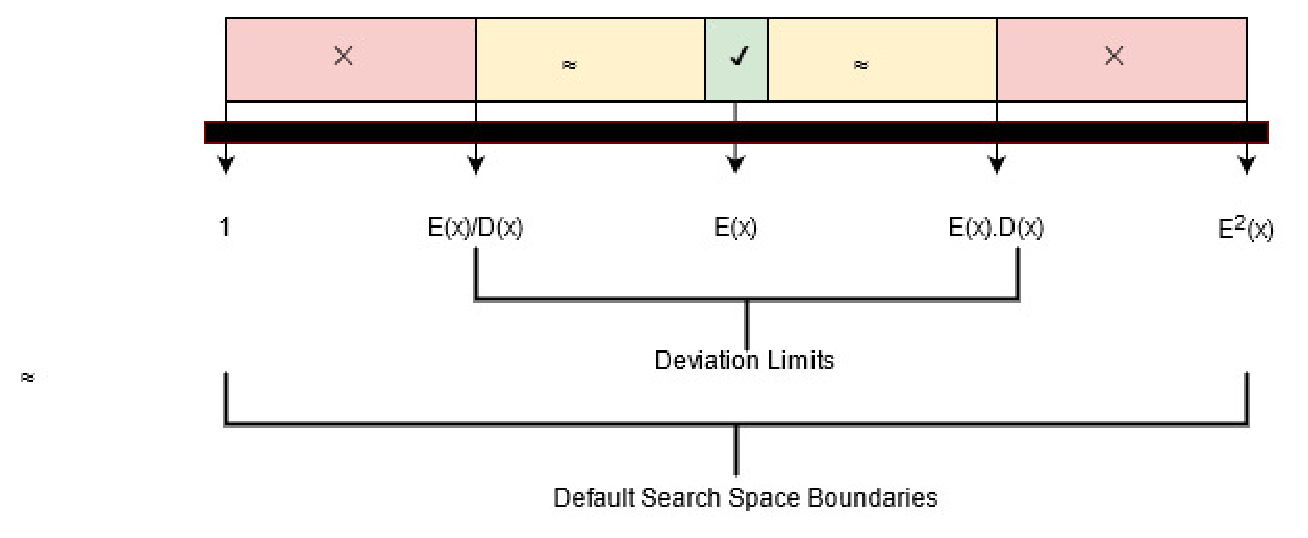
\includegraphics[scale=0.5]{bar.eps}
			\centering
			\caption{Search space boundaries and deviation limits relative to the expectation $E(x)$.}
		\end{figure}
		\item The construction of the search space is analogous to placing ticks(as shown in the figure) on a ruler as shown in the figure. The bigger ticks are the terms from the class $F_k(x)$ to which $E(x)$ belongs. 
		\item The outermost ticks are by default boundary limits, $B_l$ , lower boundary limit and $B_u$, upper boundary limit while the inner ticks are constructed by recursively halving the intervals between existing ticks. These boundaries limit the search space of possible models.
		\item The recursion terminates after a defined number of steps, which can be configured before the model generation step. The default, however, is two steps. Each new tick corresponds to a new term and is added to the search space. Practically, this is achieved by averaging the exponents of adjacent terms that are already in the search space. We denote the set of exponents of the terms already in the search space as $I_k \subset  Q$, which means we can define the search space up to this point as $$ {f(x)  \epsilon   F(x)  |  i_k  \epsilon I_k} $$. By introducing smaller ticks we can increase the resolution even further. 
		\item In contrast to the bigger ticks, smaller ticks are constructed by multiplying the terms from the class $F_k(x)$ that are already elements of the search space with terms from $F_{k-1}(x)$.
		\item As a rule of thumb and a default choice, the first term we select from $F_{k-1}(x)$ has an exponent of 1. We can then expand this selection as needed by incrementing and decrementing the exponent by a step of 1, 1/2, 1/3, and so on. 
		\item Selecting more terms from $F_{k-1}(x)$ increases the search space resolution, which incurs more overhead and is not always needed. We do not consider any terms from a class lower than $F_{k-1}(x)$ because it would result in ticks that are too fine-grained to characterize significant deviations.
		\item Finally, we multiply each term in the search space with a coefficient placeholder a and add another coefficient placeholder c, such that each term $f(x)$ becomes a function $c + a * f(x)$. Both coefficients will be instantiated when fitting the functions in the search space to actual measurements.
	\end{itemize}
	
	
	This offers both simplicity and flexibility to the user. Users can choose to define the deviation limit. Though it causes a tradeoff between speed and accuracy. Defining the deviation limit can increase the processing time.
	\newline \newline
	\subsubsection{Validate expectations}
	
	After the expectations (in terms of big O notation) are accepted, for transforming the generated models accordingly by, 
	\begin{itemize}
		\item Isolating the leading order term in a model and;
		\item Stripping off its coefficient.
	\end{itemize}
	
	To make it easy for the user to understand the results, the divergence model is designed to be $$ \delta=\frac{G(x)}{E(x)}$$ where G(x) is a generated model and E(x) is an expectation input by the user. Bug in its implementation, a bug in the algorithm, an unrealistic expectation, a constraint of the underlying architecture, or a combination of several factors can cause a severe divergence.
	\newline \newline
	We can now also verify the compliance of the actual behavior with the optional cross-function rules (Cross-functions rules specify relationships between the scaling behavior of different functions) based on the generated models. Finally, if the generated models fall within the deviation limit (i.e., match the expectations either exactly or approximately), the user may instantiate them to predict the scaling limits of selected software products at specific target scales.
	\bigskip
	
	\section{Comparison Study}
	\bigskip	
	\subsection{Software Validation Testing Techniques}
	\bigskip
	The three software validation techniques: regression testing, traceability analysis and hazard analysis are applicable in different conditions of software development, and each method has its own set of advantages and disadvantages.
	
	\bigskip
	
	\subsubsection{Based on Life-Cycle Model}
	
	Hazard analysis places emphasis on recognizing risks early and placing the necessary safe-guards against them. Such a testing technique would be especially suitable for a spiral life cycle model, as a spiral life cycle model places emphasis on identifying risks early in the software development process. 
	
	Traceability analysis requires continuous tracing of the requirements and analyzing the relationships among them. Using such a technique for an agile life cycle model would be beneficial, as in agile model, requirements are continuously added throughout the development and it is necessary to backtrace the new requirements with the old ones to ensure that there is no conflicting functionality.
	
	Regression testing works on the principle of repeatedly verifying and validating a suite of test cases to ensure that newly added functionalities do not compete with the already tested ones. This is again suitable for the agile life cycle model which is iterative in nature.
	
	\bigskip
	
	\subsubsection{Based on Documentation}
	
	Hazard analysis can often be distilled into a simple hazard table that defines the potential hazards and their respective safety constraints. As a result, hazard analysis is not documentation intensive.
	
	Traceability matrix, on the other hand, is based on a thorough definition of the various requirements and their relationships. This often requires defining several different types of use cases and designs. As seen in Putro et al \cite{trace}, there were various types of documentation such as requirements table, use case diagrams, architecture class, activity table and user interface design that needed to be defined before carrying out the analysis. As a result, the technique may become documentation intensive.
	
	Due to the iterative nature of regression testing, software validation documentation can quickly increase exponentially so as to keep track of the test cases at different stages during the development.
	
	\bigskip
	
	\subsubsection{Based on Number of Requirements}
	
	When there are a large number of software artifacts involved in the software development process, traceability analysis is most efficient due to its highly organizational nature. All the requirements are arranged in a matrix and the relationships between them are clearly defined. 
	
	Regression testing is highly expensive in cost and computation, so, as the requirements increase, the number of test cases also increase dramatically and leads to reduction in value and redundancy in testing.
	
	\bigskip
	
	\subsubsection{Based on Application}
	
	Hazard analysis, due to its emphasis on risk analysis and aversion, is suitable for safety and security critical software development projects.
	
	Regression testing can be employed for projects that are not under a time constraint and emphasis is placed on the quality of the software, as regression, due to its iterative nature, performs continuous and rigorous software quality assurance.
	
	Traceability analysis is suitable for projects with a large set of functionalities to be executed, as the various requirements are organized and traced in the matrix.
	
	Altogether, it is advantageous to use regression testing when the project emphasis is on quality. However, it is a computationally expensive testing technique and also requires large time and documentation.
	
	Hazard analysis performs a thorough risk analysis and mitigation and is concise and easy to understand. 
	
	Traceability analysis performs a thorough investigation of the various requirements involved in a software project, but consumes a large amount of documentation and is not very intuitive in nature.
	
	\subsection{Tools and Technologies}
	\bigskip
	\subsubsection{Functionality testing Tools}
	Functionality testing tool, Selenium, controls a browser remotely. It is used to simulate a user interacting with a web site, whereas JUnit acts as a framework for writing Java unit tests. For generating reports, it takes some of the grunt work out of organizing tests. JUnit will report which tests pass and which tests failed after running the tests automatically. In a situation that a test is being written for a website, JUnit tests that call APIs of Selenium. Different tools can be used based on the situation or priority of the demand.
	\bigskip
	
	\subsubsection{Maintainability testing Tools}
	FxCop is helpful for class library developers. It is interactive and a command-line tool (FxCopCmd.exe) suited for use as part of automated build processes. NDepend has more use comparatively because it gives an edge by giving code metrics for the application. It also sheds light on the architectural flaws that are usually unnoticed. It also allows the developer to compare two different versions of code. It helps in acheiveing clean concurrent programming and spots complex code at a glance.
	\bigskip
	
	\subsubsection{Usability Testing tools}
	TAW with the help of web technology performs web accessibility test by following guidelines and shows the results on the usability of a software. Hotjar uses heatmap methods to identify the number of people using a software or for how long they are using it for. This helps to understand the context behind the use of software and to what extent the components of the software are useful for.
	\bigskip
	
	\subsubsection{Security Testing tools}
	Security is one of the most important aspects of a software. OWSAP ZAP is good when it comes to DevOps/DevSecOps because of it's easier API integration and support. While BugScout has the ability to detects vulnerabilities before they reach production or a state to be hacked. Because BugScout points out the vulnerability or bugs, there won't be loss of money or time and has an edge over OWSAP ZAP
	\bigskip
	
	\subsubsection{Performance Testing Tools}
	Administration of Apache JMeter and Jetbrains dotTrace is equally easy. Both the tools can be used simultaneously for better results. Since, Apache JMeter is better suited for load testing capabilities and performance measurement and Jetbrains dotTrace for analysis of calls performed by the software.
	\bigskip
	
	\subsubsection{Continuous Verification and Validation Tools}
	The SonarQube are a de-facto standard for organizations and teams to deliver safer, better software. This performs continuous evaluation related to the maintainability, security, and reliability of the product and also shows the vulnerabilities and bugs. And it is more widely used considering it is free for some languages.
	Similarly, Cast Highlight being one of the first companies to practice continuous verification and validation tools, is widely used despite being a paid tool. When compared between both the tools, Cast Highlight has comparatively more advantages
	\bigskip
	
	\subsection{Independent Verification and Validation (IV\&V)}
	\bigskip
	\begin{figure}[H]
		\includegraphics[scale=0.3]{lifecycle.jpg}
		\centering
		\caption{V\&V Lifecycle}
	\end{figure}
	
	Validation is a type of testing performed to ensure that a product meets customer specifications. While it is indeed similar to software verification, the two should not be confused, as verification deals with whether the software meets the specification and validation is whether the specification meets customer needs. That is to say that verification checks only whether the software has been developed correctly and does not require code to be run, but validation does.
	
	\begin{itemize}
		
		\item{Independent Verification and Validation (IV\&V), is a method, in which an independent organization carries out the verification and validation of a system under development.  This is effective because the checks are performed by someone other than the developer, with a different viewpoint, thus facilitating a more stringent check. The independent tester is unprejudiced and has no presupposition about quality.
			However, IV\&V is at a disadvantage to V\&V in some ways. IV\&V teams do not entirely understand the minutia of the product, and thus, may not comprehend which parts of the system should be verified and validated, nor what kind of verification or validation may need to be performed. The testers are also secluded from the development team; this may result in out-of-date documentation references and sources. There is also the issue of communication that arises when different teams are working on the same project, in this case, the developers and the testers.}
		
		\item{IV\&V testers likely have more experience with testing, since they carry it out 24/7 vs. the development organization doing it only every so often in between development cycles. As a result of this, they are also more likely to have the latest technology and use the best methods to perform tests, and they can test more at lower prices since they essentially mass produce tests.}
		
		\item{Different levels of independence: Independent V\&V does not necessarily need to be done by a separate organization. It can be performed by a specialized team within the developing organization itself. And even when taken up by a separate organization, there might exist a specific team that sees the whole project through to completion or different teams each cycle. As such, the boundary between standard V\&V and IV\&V is a little fuzzy, since the V\&V team may know from next to nothing about the project to quite a bit about it depending on how closely associated they are with the development team.}
	\end{itemize}
	\bigskip
	
	
	\subsubsection{The Agile Model and IV\&V}
	
	
	The Agile model is highly valued for its speed and adaptability to changing customer requirements. They allow for rapid development, grant customer satisfaction, and accommodate any sorts of changes if necessary. At first, they were used in smaller systems, but now, large-scale and mission-critical systems have begun adopting this model as well. Hybrid Agile methods are designed to aid in the development of large-scale systems. However, hybrid Agile development practices and IV\&V may not be fully compatible. It should be noted that IV\&V helps the most when done starting early in the development lifecycle. On the other hand, Agile methods focus on defining things as required throughout the lifecycle rather than deciding everything early on.
	\bigskip
	Due to the incompatibility issue mentioned above, new techniques may be required for more efficient development of large-scale and mission-critical systems. Integrating the Spiral model and IV\&V may be a possible solution to fix most issues that cause the agile model to be incompatible with IV\&V.
	\bigskip
	
	\subsubsection{The Spiral Model and IV\&V}
	As mentioned in Section 3-E, the Agile model finds it difficult to accommodate the IV\&V techniques, due to the various reasons outlined above. The Spiral Model may be better suited to accommodate IV\&V techniques than the Agile model since its focus on risk analysis is greater.
	
	\bigskip
	
	In the combination of the Spiral model and IV\&V techniques, the risks analysed via the Spiral Model may be delivered to the independent testers, helping them identify more clearly, which parts to prioritise while verifying and validating. As we can see, adopting these spiral model practices into the agile model might make it more suitable to support IV\&V.
	
	\bigskip
	
	\subsubsection{Advantages and Disadvantages of IV\&V}
	
	IV\&V techniques fill in a lot of gaps that traditional testing can’t cover. For one, the team is unrelated to development, and therefore won’t have any preconceived notions of what the product was intended to look like or function as. This allows them to be more objective and unbiased while conducting tests, either positively or negatively so. Second, this can give the development team a bit of a break and take some work off their shoulders, especially in matters like coming up with test cases. This can go a long way in improving the quality of the developed software, since they can focus purely on coding and not thinking about what tests their software will need to pass. Independent teams also have the added advantage of being able to simply slightly modify tests that already exist in their repositories to meet testing requirements.
	
	\bigskip
	
	However, some of these advantages can also be drawbacks. Not knowing anything about the software can be a boon, but it can also be a bane, since this means that the testing teams don’t know what critical areas to focus on while testing the system. This sort of testing can also lead to the developers being lax since they don’t need to code to pass any specific tests. In addition, since they aren’t associated with the development team, the testers might not be up-to-date on any changed specifications that might have been introduced during the development process There is also a chance that since the testers aren’t the developers, a lack of communication can cause major misunderstandings that can set projects back by a lot. 
	
	\bigskip
	
	\subsubsection{IV\&V and Assurance Testing}
	
	In Smith et al. \cite{hazard}, the independent software validation team performed Hazard Analysis on MEXEC, the software that provides the satellite ASTERIA with autonomous control. 
	
	But instead of using the tradition software validation practices, they employed assurance cases to present critical information like potential hazards in the working of the autonomous software. 
	
	When they presented their results to the MEXEC development team, however, they noticed that the usage of assurance cases to document the hazard analysis did not aid in the understanding of the analysis, and resulted in a communication gap between the developers and the validators. 
	
	This, as discussed before, is a common disadvantage of IV\&V. This issue could have been mitigated by adopting the reference model \cite{refmod}. The assurance case approach could have been well documented in the reference model to reduce ambiguity and bridge the communication gap.
	
	
	\bigskip
	\section{Future Work}
	\bigskip
	\subsection{Future Development in Software validation}
	\bigskip
	There are several future developments that can be made in the field of software validation. 
	
	Despite its assurance on well validated software projects, regression testing is still a very intensive, reduntant and costly technique. Future innovations can help improve test case selection strategy and reduce its cost. Robust algorithms that define the best test case suite can be developed, and artificial intelligence can choose the best test suite on a case-by-case basis. 
	
	Hazard analysis is not a well developed or a well used validating technique. It can be improved by presenting the system information in a formal model such as the Model Based Systems Engineering (MBSE).
	
	Traceability analysis can be automated with the help of sophisticated machine learning algorithms that continuously perfrom tracing to ensure that the specified requirements are satisfied.
	
	\subsection{Future development in Technologies and Tools}
	\bigskip
	There is more demand for quality software. A company's stand in the market depends on its quality. But using traditional methods of software validation can be costly, time consuming and less quality. The future is in the automation of this phase. Based on data exploits, the future verification and validation tools will include business intelligence, and learn or adapt themselves about the software and improve software quality in a dynamic way. This will be more cost efficient over the long run. 
	
	\subsection{Future Development in IV\&V}
	\bigskip
	There is plenty of future work to be done in the field of IV\&V. We have outlined some of the problems in this field in our report, with the help of various research papers. Future solutions may include new techniques or entirely new technologies. Another solution that will go a long way in improving the efficiency of validation practices, is better computer infrastructure. 
	
	The plan of action must be to explore options to resolve the hybrid Agile and IV\&V incompatibilities from two viewpoints: the developer and IV\&V. From the developer’s side, adjusting the hybrid Agile lifecycle can supply essential information earlier in the project, at a time when it is more useful to validate. From the IV\&V side, new techniques could be developed, which would perform verification and validation incrementally, and keep up with the hybrid Agile methodology.
	
	We are already seeing improvements in this field, with current techniques already easily outdoing older techniques both in terms of finance and of efficiency. We must endeavour to allow for as much out-of-the-box functionality as possible, while also remaining flexible enough to match the current and projected future needs of customers. Increasing the efficiency of validation activities in any way possible will be a huge step in the software development process. Automation may be a feasible way to pull this off, with major development expected from the fields of AI and machine learning in the near future. This will likely eliminate most problems that currently hamper the validation process, since so many stem from human errors.
	
	Automation can manage both the software and new builds that are vulnerable to defects and manual errors. Agility in testing means using the latest technologies since it’s something that requires flexibility. Agile testing places emphasis on constant testing, rectifying bugs in real time, and constant feedback. Its final aim is to reduce the time of the release of the product into the market.
	
	\subsection{Future Development in Validation Algorithms}
	Validation algorithms are incredibly useful tools that helps a developer to achieve the required task by just giving in an initial input. These algorithms helps a developer to obtain the results faster, error-free. There is a huge scope in these algorithms because a company or a product will get edge over its competition if it has effective algorithms. 
	\newline\newline
	In future, time efficient, cost efficient, and less complex algorithms will be created.
	\bigskip
	There is plenty of future work to be done in the field of IV\&V. We have outlined some of the problems in this field in our report, with the help of various research papers. Future solutions may include new techniques or entirely new technologies. Another solution that will go a long way in improving the efficiency of validation practices, is better computer infrastructure.
	\bigskip
	\section{Conclusion}
	\bigskip
	
	We reviewed literature in the field of software validation to analyse recent developments in the domain. Our study included the tools and technologies used in software validation, software validation testing techniques including regression testing, traceability analysis, and hazard analysis, Independent Verification and Validation (IV\&V), as well as software validation algorithms.
	
	We analyzed various validation testing techniques such as regression testing, traceability analysis and hazard analysis and compared their merits and demerits. We reviewed various tools and technologies available in software validation today. We also reviewed the IV\&V practice, and assessed its various merits and demerits, especially in the application to the agile model, and saw how its implementation can be improved by a reference model. Lastly, we analyzed the scaling algorithm to improve the quality of software validation.
	
	
	Validation is one of the most important tasks in the software development process, a task that has the potential to reduce rework significantly. It is also very time-consuming. From the research papers we studied, we concluded that while there is considerable research that is being performed in this field, there are a lot of improvements in efficiency, reliability, speed, and ability to be integrated with advanced software development methods that are yet to be made.
	
	
	
	\pagebreak 
	\newpage
	
	\bibliographystyle{IEEEtran}
	\bibliography{validation}

	\pagebreak
	\appendix
	
	\begin{table*}[h]
		\centering
		\begin{tabular}{|p{1cm}||p{1.5cm}|p{1.5cm}|p{1.25cm}|p{3cm}|}
			
			\hline
			\multicolumn{5}{|c|}{Functional Testing Tools} \\
			\hline
			Name of Tool & Type & License & Technology &Description\\
			\hline
			JUnit  & XUnit tools  & Open source &Java&   The most famous XUnit framework for Java \\
			\hline
			Selenium & Capture and replace tool &  Open source  & Web   &Selenium Web Allows creating automated tests for web applications; tests can be recorded or scripted in multiple languages\\
			\hline
		\end{tabular}
		\caption{Functional Testing Tools}
	\end{table*}
	
	
	\begin{table*}[h]
		\centering
		\begin{tabular}{|p{1cm}||p{1.5cm}|p{1.5cm}|p{1.25cm}|p{3cm}|}
			\hline
			\multicolumn{5}{|c|}{Maintainability Testing Tools} \\
			\hline
			Name of Tool & Type & License & Technology &Description\\
			\hline
			FxCop  & Static analysis Tools  & Free & NET &   Analyzes managed code assemblies and reports information about flaws \\
			\hline
			NDepend & Static analysis Tools &  Commercial  & NET  &Offers metrics related to the quality of the source code\\
			\hline
		\end{tabular}
		\caption{Maintainability Testing tools}
	\end{table*}
	
	\pagebreak 
	
	\begin{table*}
		\centering
		\begin{tabular}{|p{1cm}||p{1.5cm}|p{1.5cm}|p{1.25cm}|p{3cm}|}
			\hline
			\multicolumn{5}{|c|}{Usability Testing Tools} \\
			\hline
			Name of Tool & Type & License & Technology &Description\\
			\hline
			TAW  & Static analysis tools  & Free & Web &   Web accessibility test with WCAG 2.0 guidelines (A,AA)\\
			\hline
			Hotjar & Usability testing and inspection tools &  Commercial  & Web  &Complete analytics and feedback tool that helps users identify opportunities for Improvement (heat maps, visitor recordings, surveys and more)\\
			\hline
		\end{tabular}
		\caption{Usability Testing Tools}
	\end{table*}
	
	
	\begin{table*}
		\centering
		\begin{tabular}{|p{1cm}||p{1.5cm}|p{1.5cm}|p{1.25cm}|p{3cm}|}
			\hline
			\multicolumn{5}{|c|}{Security Testing Tools} \\
			\hline
			Name of Tool & Type & License & Technology &Description\\
			\hline
			OWASP ZAP  & Security and Pentesting tools  & Open source & Web &   Penetration testing tool to find a variety of security vulnerabilities in
			web apps, even during the development and testing phases\\
			\hline
			BugScout & Static analysis tools &  Commercial  & Java, .NET, and PHP  &Detects potential security risks in applications before they reach production and can be hacked\\
			\hline
		\end{tabular}
		\caption{Security Testing Tools}
	\end{table*}
	
	
	\pagebreak 
	
	\begin{table*}
		\centering
		\begin{tabular}{|p{1cm}||p{1.5cm}|p{1.5cm}|p{1.25cm}|p{3cm}|}
			\hline
			\multicolumn{5}{|c|}{Performance Testing Tools} \\
			\hline
			Name of Tool & Type & License & Technology &Description\\
			\hline
			Apache JMeter  & Performance testing tools  & Open source & Web & Provides load testing capabilities and performance measurement for functional behavior\\
			\hline
			Jetbrains dotTrace & Performance testing tools &  Commercial  & .NET & Performance profiler provides analysis of calls\\
			\hline
		\end{tabular}
		\caption{Performance testing Tools}
	\end{table*}
	
	\pagebreak	
	\begin{table*}[t]
		\centering
		\begin{tabular}{|p{1cm}||p{1.5cm}|p{1.5cm}|p{1.25cm}|p{3cm}|}
			\hline
			\multicolumn{5}{|c|}{Continuous Verification and Validation Tools} \\
			\hline
			Name of Tool & Type & License & Technology &Description\\
			\hline
			Cast Highlight  & Continuous verification and validation tools  & Commercial & Analyzes 18 different languages & Cast is one of the first companies that has started with the quality measurements, and Highlight is one of its tools that is integrated with the rest of the lifecycle tools, allowing assess and track application portfolio health, identifying security vulnerabilities and making application benchmarks\\
			\hline
			SonarQube & Continuous verification and validation tools &  Free for some languages and commercial for others  & Analyzes 20 different languages &It is one of the references and most used tools in the continuous validation of software quality. It obtains an evaluation related to the maintainability, security, and reliability of the product, detecting code smells, vulnerabilities, and bugs. It is integrated into the development cycle and allows validating the quality of any change that is made throughout the life of the product\\
			\hline
		\end{tabular}
		\caption{\label{tab:table-name}Continuous Verification and validation tools} 
	\end{table*}
	
	\pagebreak
	
	
	
\end{document}